\section{Problemas não resolvíveis}

\begin{description}

\item[] \textbf{OBS:} Nem sempre um sistema de equações é resolvível:

\item[] No conjunto:

\begin{enumerate}[S.1:]

\item As duas equações são idênticas. Qualquer ponto satisfazendo uma equação satisfaz outra. Assim, o sistema tem infinitas soluções (linearmente independentes).

\item Inconsistente se lado esquerdo de uma das equações for eliminado por combinação linear das outras equações, enquanto o lado direito permanece diferente de zero.

\item Duas incógnitas e três equações nunca são satisfeitas simultaneamente.

\end{enumerate}

\begin{figure}[!ht]
 \centering
 \begin{minipage}[c]{0.8cm}
 S.1:
 \end{minipage}
 \begin{minipage}[c]{3cm}
    \[
     \left\{ \begin{array}{rrrrr}
      -x & + & y & = & 1 \\
      -2\,x & + & 2\,y & = & 2
     \end{array} \right.
    \]
 \end{minipage}\hspace*{2cm}
 \begin{minipage}[c]{5cm}
    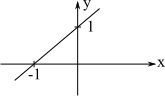
\includegraphics[scale=0.8]{capitulos/capitulo4/figuras/prob_nao_resol1.png}
    \label{fig:prob_nao_resol1}
 \end{minipage}
\end{figure}

\begin{figure}[!ht]
 \centering
 \begin{minipage}[c]{0.8cm}
 S.2:
 \end{minipage}
 \begin{minipage}[c]{3cm}
    \[
     \left\{ \begin{array}{rrrrr}
      -x & + & y & = & 1 \\
      -x & + & y & = & 0
     \end{array} \right.
    \]
 \end{minipage}\hspace*{2cm}
 \begin{minipage}[c]{5cm}
    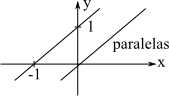
\includegraphics[scale=0.8]{capitulos/capitulo4/figuras/prob_nao_resol2.png}
    \label{fig:prob_nao_resol2}
 \end{minipage}
\end{figure}

\begin{figure}[!ht]
 \centering
 \begin{minipage}[c]{0.8cm}
 S.3:
 \end{minipage}
 \begin{minipage}[c]{3cm}
    \[
     \left\{ \begin{array}{rrrrr}
      -x & + & y & = & 1 \\
      x & + & 2\,y & = & -2 \\
      2\,x & - & y & = & 0
     \end{array} \right.
    \]
 \end{minipage}\hspace*{2cm}
 \begin{minipage}[c]{5cm}
    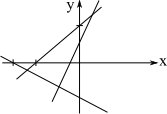
\includegraphics[scale=0.8]{capitulos/capitulo4/figuras/prob_nao_resol3.png}
    \label{fig:prob_nao_resol3}
 \end{minipage}
\end{figure}

\item[] Solução única (condições necessárias):

\begin{itemize}

\item Número de equações igual ao número de incógnitas.

\item Equações são L.I. (linearmente independentes)

\end{itemize}

\end{description}